\section{Datasets \& Data Generation}
\label{sec:dataset}

In this section, we present the datasets and data-generation frameworks used throughout the paper. As a key contribution, we introduce \datakit (\cref{subsec:datakit}), a publicly available framework to generate the most diverse, realistic, and scalable synthetic datasets for Power Flow (PF), Optimal Power Flow (OPF), and State Estimation (SE). Additionally, we describe two widely used benchmark datasets for PF and OPF (\cref{subsec:benchmark_data}), which we use to compare \genco against existing state-of-the-art models under standard evaluation settings in \cref{subsec:pf} and \cref{subsec:opf}. Finally, we compare the diversity of \datakit-generated data against real SCADA data from Hydro-Québec in \cref{subsec:comparison_data_hq}.







\subsection{Data Generation with \datakit}
\label{subsec:datakit}
We utilize \datakit to generate large PF and OPF datasets. \datakit unifies and advances state-of-the-art synthetic grid data generation methods, uniquely generating realistic off-nominal operating condition samples for PF and diverse generator costs for OPF. We here provide a short overview of the main features of \datakit. For a detailed technical description of the pipeline, runtime analysis, and exhaustive comparisons against other libraries (summarized in \cref{tab:comparison}), we refer to the \datakit technical report~\cite{puech2025gridfmdatakitv1pythonlibraryscalable}.


\begin{table*}[t]
\centering
\small
\resizebox{\textwidth}{!}{
\begin{tabular}{l c c c c c c c c}
& & \multicolumn{3}{c}{Load Variations} & & & & \\
\cmidrule(lr){3-5}
Library & Grid Size &
\makecell{Spatial\\Correlation} &
\makecell{from Real\\Profiles} &
Diverse$^*$ &
\makecell{Higher-order N-k ($k>2$)\\Topology Variations} &
\makecell{Admittance\\Variations} &
\makecell{Generator Profile\\Variations} &
\makecell{Off-Nominal\\Operating Scenarios} \\
\midrule

\multicolumn{9}{c}{\textbf{Power Flow (PF) Datasets}} \\
\midrule
\datakit-pf~\cite{puech2025gridfmdatakitv1pythonlibraryscalable} & 30K & \cmark & \cmark & \cmark & \cmark & \cmark & \cmark & \cmark \\
\pfdelta~\cite{NEURIPS2025_d000ef56} & 2K & \xmark & \xmark & \cmark & \xmark & \xmark & \cmark & \cmark \\
PFNet~\cite{lin2024powerflownet} & 6K & \cmark & \xmark & \xmark & \xmark & \cmark & \xmark & \xmark \\
\midrule

\multicolumn{9}{c}{\textbf{Optimal Power Flow (OPF) Datasets}} \\
\midrule
\datakit-opf~\cite{puech2025gridfmdatakitv1pythonlibraryscalable} & 10K & \cmark & \cmark & \cmark & \cmark & \cmark & \cmark & --- \\
OPFData (CANOS)~\cite{piloto2024, lovett2024opfdatalargescaledatasetsac} & 14K & \cmark & \xmark & \xmark & \xmark & \xmark & \xmark & --- \\
OPF-Learn~\cite{opflearn} & 118 & \xmark & \xmark & \cmark & \xmark & \xmark & \xmark & --- \\
PGLearn~\cite{pglearn} & 24K & \cmark & \xmark & \cmark & \xmark & \xmark & \xmark & --- \\
PowerGraph~\cite{varbella2024powergraph} & 118 & \cmark & \cmark & \xmark & \xmark & \xmark & \xmark & --- \\
\bottomrule
\end{tabular}}
\caption{Comparison of PF and OPF data generation libraries. $^*$Diverse load variations denote load scenarios that extend beyond uniform perturbations around nominal operating points and beyond simple global scaling of all loads. OPF datasets do not contain off-nominal scenarios, as OPF solutions have to satisfy all operational constraints (e.g., thermal and voltage limits).}
\label{tab:comparison}
\end{table*}

\subsubsection{Grid Support and Scalability}
\datakit uses PowerModels.jl~\cite{powermodels} with distributed Julia~\cite{julia} runtimes through JuliaCall~\cite{juliacall} to scale to networks of up to 30{,}000 buses for PF and 10{,}000 buses for OPF, supporting MATPOWER~\cite{matpower} (e.g., all PGLib grids~\cite{pglib}), PSS$^{\circledR}$E~\cite{siemens_psse_v34}, and ENTSO-E's CGMES~\cite{entsoe_cim_network_model_management_guide} formats. Importantly, the library can be used to generate data for real grids, as we demonstrate for the $\sim$1{,}200-bus Hydro-Qu\'ebec (HQ1200) network.\\

The generation is highly parallelized; as shown in \cref{tab:scalability}, generating $\sim$200,000 samples for the IEEE 118-bus system requires under 20 minutes for PF and roughly 2 hours for OPF\footnote{using 20 cores of an AMD EPYC 7763 CPU @ 2.45 GHz.}. Moreover, the convergence rate exceeds 97\% across all grid sizes for PF thanks to the use of robust solvers and our load sampling technique, compared to approximately 75\%~\cite{hitandrun} for methods utilizing hit-and-run sampling that uniformly explore the feasible load space, such as OPF-Learn~\cite{opflearn} and \pfdelta~\cite{NEURIPS2025_d000ef56}.
\begin{table}
\centering
\caption{Time required to generate approximately 200,000 samples with N-1 topology perturbations for different grid sizes. The reported number of samples corresponds to successfully converged samples. Refer to~\cite{puech2025gridfmdatakitv1pythonlibraryscalable} for details on runtimes.}\label{tab:scalability}
\resizebox{1.0\linewidth}{!}{%
\begin{tabular}{lccc}
\hline
Grid name & \makecell{Number of\\converged samples [-]} & 
\makecell{CPU\\Core-hours [-]} & 
\makecell{Convergence\\rate [\%]} \\
\hline
\multicolumn{4}{c}{\textbf{Power Flow (PF)}} \\
\hline
IEEE 24 bus  & 199,540  & 2.69      & 99.77     \\
IEEE 118 bus & 199,339  & 6.44      & 99.67     \\
GOC 2k bus    & 198,858  & 247.55    & 99.43     \\
GOC 10k bus   & 199,880  & 1,384.24  & 99.94     \\
\hline
\multicolumn{4}{c}{\textbf{Optimal Power Flow (OPF)}} \\
\hline
IEEE 24 bus  & 190,387  & 21.33     & 95.19     \\
IEEE 118 bus & 197,769  & 46.10     & 98.88     \\
GOC 2k bus    & 198,308  & 1,103.67  & 99.15     \\
GOC 10k bus   & 195,920  & 3,628.01  & 97.96     \\
\hline
\end{tabular}}
\end{table}

\subsubsection{Load Scenarios}
Public grid datasets rarely provide bus-level load trajectories due to the sensitive nature of operational data. Consequently, synthetic datasets typically rely on a single nominal operating point and generate scenarios through artificial perturbations. Existing approaches either randomly perturb the base load independently at each bus~\cite{lin2024powerflownet, piloto2024, lovett2024opfdatalargescaledatasetsac}, or sample loads randomly in the feasible space~\cite{NEURIPS2025_d000ef56,opflearn}, which may fail to preserve realistic spatial and temporal load correlations. To address these limitations, we implement a hybrid perturbation strategy that combines realistic system-level demand evolution with local bus-level diversity. At time $t$, a global scaling factor \texttt{ref}$_t$ is derived from real aggregated profiles provided in \datakit, e.g., ERCOT's 2025 hourly system-level load published by the EIA~\cite{EIA_ERCOT_2025}, or other user-provided aggregated load profiles. For nominal loads $p_i$ and $q_i$ at bus $i$, the perturbed load is:
\begin{equation}
\label{eq:scaling}
    \tilde{p}_{i,t} = p_i \cdot \texttt{ref}_t \cdot \epsilon^p_{i,t}, \quad \tilde{q}_{i,t} = q_i \cdot \texttt{ref}_t \cdot \epsilon^q_{i,t}
\end{equation}
where $\epsilon^p_{i,t}, \epsilon^q_{i,t} \sim \mathcal{U}(1 - \sigma, 1 + \sigma)$ are independent local perturbation factors sampled from a uniform distribution over $[1-\sigma,1+\sigma]$, introducing per-bus variability, while $\texttt{ref}_t$ captures the temporal evolution of the aggregated demand.

\subsubsection{Topology and Admittance Perturbations}
Unlike all other libraries that are limited to N-1~\cite{lin2024powerflownet, lovett2024opfdatalargescaledatasetsac, piloto2024, opflearn, pglearn, varbella2024powergraph} or up to N-2~\cite{NEURIPS2025_d000ef56} contingencies, \datakit supports arbitrary N-k topology perturbations through either exhaustive enumeration or rejection sampling (to avoid islanding). Admittance variations are introduced by scaling branch resistances and reactances by random factors sampled from a uniform distribution.

\subsubsection{Generator Setpoints and Data Modes}
\label{subsubsec:gen_setpoints}

\paragraph{OPF mode.}
Generator setpoints are computed by solving AC-OPF on the perturbed topology. To ensure generalizability across market conditions, \datakit permutes or randomly scales generator cost coefficients prior to solving, introducing dispatch diversity, absent in fixed-cost libraries.

\paragraph{PF mode.}
Base generator setpoints are obtained by solving AC-OPF on the base topology (without perturbations, but accounting for load, admittance, and generator cost variations). Then, N-k topology perturbations are applied, and AC-PF is solved \textit{without} re-optimizing dispatch, producing realistic off-nominal operating states that may violate OPF constraints (e.g., line overloads, voltage limits). This yields a balanced mix of points within and outside normal operating limits, reflecting realistic system behavior where OPF determines generator dispatch under nominal conditions and unexpected changes may lead to violations.


\subsection{Benchmark Datasets}
\label{subsec:benchmark_data}
To benchmark \genco against existing state-of-the-art neural solvers (\cref{subsec:pf} and~\ref{subsec:opf}), we additionally leverage two widely used benchmark datasets: \pfdelta~\cite{NEURIPS2025_d000ef56} for PF and OPFData~\cite{lovett2024opfdatalargescaledatasetsac} for OPF. While these datasets enable direct comparison with existing neural solvers under standard evaluation settings, they remain limited in several important aspects. In particular, they do not provide DC-PF or DC-OPF solutions, preventing direct comparison with classical DC solvers under the same evaluation settings. More importantly, their limited scenario diversity prevents studying model generalization under diverse topology perturbations, varying generator costs, contingency scenarios, or admittance perturbations. Therefore, \datakit, which addresses these limitations, is used for all other experiments.
\\\\
\textbf{\pfdelta}~\cite{NEURIPS2025_d000ef56} is a dataset of solved PF problems with load scenarios sampled via hit-and-run to explore the feasible load space, permuted generator costs, N-1 and N-2 topology perturbations, and scenarios generated by solving OPF excluding selected inequality constraints to obtain off-nominal operating conditions. Unlike \datakit, it does not offer real load profiles, admittance variations, or higher-order topology perturbations; but it enables comparison against state-of-the-art PF models (GNS~\cite{DONON2020106547}, CANOS-PF~\cite{piloto2024}, PFNet~\cite{lin2024powerflownet}).
\\\\
\textbf{OPFData} is a widely used~\cite{arowolo2025, hedgeopf2025,piloto2024, lumina2026, yang2026gridsfm} dataset for OPF with N-1 topology perturbations. Despite being one of the largest publicly available OPF datasets, it has various limitations: (i) load scenarios are generated by independently scaling each load with a uniform factor in $[0.8, 1.2]$, limiting load diversity and realism; and (ii) fixed generator cost parameters, which restrict generator setpoint diversity by effectively forcing low-cost generators to operate at capacity across most scenarios. However, it enables direct comparison of \genco with HH-MPNN~\cite{arowolo2025}, the currently best-performing open-source model using this dataset.





\subsection{Validation of Synthetic Data Against Hydro-Québec Real-World SCADA Dataset}
\label{subsec:comparison_data_hq}


\begin{figure}
\centering
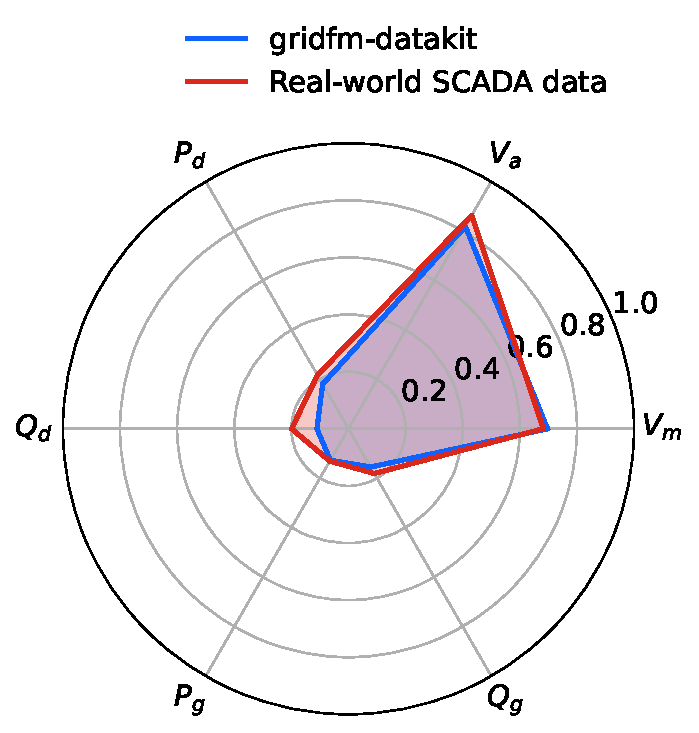
\includegraphics[width=0.7\linewidth]{figures/data/spider_plot_entropy_hq.pdf}
\caption{Normalized mean feature entropy of real-world SCADA PF data from HQ1200 and synthetic PF data generated for HQ1200 using \datakit. Values close to one indicate higher diversity, with one corresponding to a uniform distribution. Features are: $V_m$/$V_a$: bus voltage magnitudes/angles; $P_g$/$Q_g$: active/reactive power generation; $P_d$/$Q_d$: active/reactive power demand.} 
\label{fig:spider_hq1200}
\end{figure}


A key trade-off in data generation lies between covering a broad range of operating conditions and avoiding unrealistic samples that can destabilize training or distract from the regimes that matter. To assess the diversity of the data generated with \datakit, we compare it against real-world SCADA measurements from the Hydro-Québec (HQ) transmission network\footnote{Beyond the validation against real-world SCADA data presented here, a broader data diversity comparison with existing PF and OPF datasets is provided in the \datakit technical report~\cite{puech2025gridfmdatakitv1pythonlibraryscalable}.}, referred to as HQ1200, using normalized Shannon entropy\footnote{Standard deviation overestimates variability when features take few discrete values (e.g., $P_g$ switching between zero and its upper bound). In contrast, Shannon entropy remains low when samples concentrate in a small region of the admissible space and increases only when the empirical distribution spreads across multiple populated regions.} across key grid features, following~\cite{puech2025gridfmdatakitv1pythonlibraryscalable, hedgeopf2025}. Values near zero indicate little variability, whereas values approaching one correspond to broad and nearly uniform exploration of the feature’s admissible range.\\

Real topologies and PF data were extracted from SCADA at 30-minute intervals over the year 2024, forming a dataset of network snapshots that comprises approximately 1,200 nodes and 1,600 branches after aggregating the full HQ transmission network ($\sim$2,600 nodes). These snapshots are the output of the state estimator, and each power-flow solution has been verified for convergence with the PSS$^{\circledR}$E software~\cite{siemens_psse_v34}. We compute the normalized Shannon entropy on a set of 15,000 samples and compare it with the entropy obtained from the same number of samples generated with \datakit on a representative HQ1200 base topology in \cref{fig:spider_hq1200}. Only the base topology and grid parameters are given as input to \datakit, which then generates load, topology, admittance, and generator cost scenarios. \\

The results indicate that the entropy of the synthetic data closely matches that of the real-world data, except for reactive power demand, which is slightly more diverse in the real data. This gap is consistent with reduced power factor variability in \datakit, resulting from the joint scaling of active and reactive demands through a global scaling factor (while only the local scaling factors differ between active and reactive loads; see \cref{eq:scaling}).\\




\begin{boxH}
\paragraph{Takeaways.}
\begin{itemize}
\item \datakit enables fast and scalable generation of diverse, realistic PF and OPF datasets, generating 200,000 IEEE 118-bus samples in less than 20 minutes for PF and less than 2 hours for OPF using 20 CPU cores, while scaling to 10k-bus systems for OPF and 30k-bus systems for PF.
\item \datakit addresses key limitations of existing PF and OPF datasets by generating realistic off-nominal PF operating conditions and OPF scenarios with diverse generator cost coefficients.
\item The diversity of \datakit-generated data closely aligns with that of real Hydro-Québec SCADA data on the HQ1200 network.
\end{itemize}
\end{boxH}


